\documentclass[aps,pra,twocolumn,superscriptaddress]{revtex4-2}
\usepackage{graphicx}% Include figure files
\usepackage{dcolumn}% Align table columns on decimal point
\usepackage{bm}% bold math
\usepackage{amssymb}
\usepackage{amsmath}
\usepackage{natbib}
\usepackage{hyperref}% add hypertext capabilities
\usepackage{siunitx}
%\usepackage[caption=false]{subfig}
\usepackage{subcaption}%replaces subfig
%\usepackage{caption}
\usepackage[export]{adjustbox}
\usepackage{upgreek} %upright greek letters
\usepackage{xfrac} %small fractions
\usepackage{physics}
\usepackage{xcolor} %for inkscape colors
%\usepackage[mathlines]{lineno}% Enable numbering of text and display math
%\linenumbers\relax % Commence numbering lines
\usepackage{accents}
\usepackage{comment}

%%plotting packages and mods
\usepackage{tikz-network} %for coupling graphs
\SetVertexStyle[TextColor = white, TextFont = \tiny, LineWidth=0pt]
\usepackage{tikz}
\usepackage{pgfplots} % LaTeX
\usepgfplotslibrary{colormaps} %colormaps
\usepgfplotslibrary{groupplots} %for experimental section. Remove if section is upgraded
\pgfplotsset{/pgfplots/colormap={PRGn}{rgb255(-1)=(64,0,75) rgb255(0)=(246,246,246) rgb255(1)=(0,68,27)}} %colormap for gradients
%\usepgfplotslibrary{groupplots}
%\pgfplotsset{compat = newest}
\pgfplotsset{compat=1.17}
\pgfkeys{/pgf/number format/.cd,1000 sep={}}

%%read coordinates for 3D matrix
\makeatletter
\newcommand*\readcoords[1]{\@@input #1 }
\makeatother
\newcommand{\ASN}[1]{{\color{red}{#1}}}
%%make captions justified
\captionsetup[sub]{justification = raggedright, singlelinecheck = false, position=top} %subcaptions on top lect corner
\captionsetup{font=small, justification=Justified, format=plain,singlelinecheck = false} 
\captionsetup[figure]{font=small,justification=Justified,format=plain}%captions on bottom left






\begin{document}
%% Custom commands
\newcommand{\jdae}[1]{{\textcolor{blue}{#1}}}
\newcommand{\rg}[1]{{\textcolor{purple}{#1}}}
\newcommand{\delete}[1]{{\textcolor{red}{#1}}}



\title{ Engineering spin-spin interactions with optical tweezers in trapped ions}

\author{J. D. Arias Espinoza}\affiliation{Van der Waals-Zeeman Institute, Institute of Physics, University of Amsterdam, 1098 XH Amsterdam, the Netherlands}
\author{M. Mazzanti}\affiliation{Van der Waals-Zeeman Institute, Institute of Physics, University of Amsterdam, 1098 XH Amsterdam, the Netherlands}
\author{R. X. Sch{\"u}ssler}\affiliation{Van der Waals-Zeeman Institute, Institute of Physics, University of Amsterdam, 1098 XH Amsterdam, the Netherlands}
\author{Z. Wu}\affiliation{Van der Waals-Zeeman Institute, Institute of Physics, University of Amsterdam, 1098 XH Amsterdam, the Netherlands}
\author{K. Fouka}\affiliation{Van der Waals-Zeeman Institute, Institute of Physics, University of Amsterdam, 1098 XH Amsterdam, the Netherlands}
\author{P. Corboz}\affiliation{QuSoft, Science Park 123, 1098 XG Amsterdam, the Netherlands}\affiliation{Institute for Theoretical Physics, Institute of Physics, University of Amsterdam, Science Park 904, 1098 XH Amsterdam, the Netherlands}
\author{R. Gerritsma}\affiliation{Van der Waals-Zeeman Institute, Institute of Physics, University of Amsterdam, 1098 XH Amsterdam, the Netherlands}
\author{A. Safavi Naini}\affiliation{QuSoft, Science Park 123, 1098 XG Amsterdam, the Netherlands}\affiliation{Institute for Theoretical Physics, Institute of Physics, University of Amsterdam, Science Park 904, 1098 XH Amsterdam, the Netherlands}


\begin{abstract}
We consider the use of optical tweezers to engineer the soundwave spectrum of trapped ion crystals. We show that this engineering allows for powerful new ways to tune the interactions and connectivity of the ion-qubits. We calculate that realistic tweezer settings may be used to obtain particular spin-spin interactions between the ion qubits. These may be used to implement quantum simulation of spin models. We demonstrate how optimal tweezer patterns may be obtained, show examples of spin-spin interaction patterns of interest both in one- and two-dimensional ion crystals and discuss the possible experimental implementation.
\end{abstract}

\maketitle

\section{Introduction}
%\jdae{Move to intro:A powerful feature of our approach is the capability of controlling the decay strength of power law interactions \(1/|\rho|^{\alpha}\) in a linear ion chain. This will allow quantum dynamical processes such as MBL, Scrambling, ....}

Trapped-ions are one of the leading platforms for quantum computation and quantum simulation~\cite{Ballance2016,Gaebler2016,Zhang2017}. Numerous experiments have demonstrated the ability of the analog trapped-ion quantum simulator to emulate the dynamics of models relevant to quantum magnetism~\cite{Friedenauer:2008,Lanyon:2011,Cirac:2012,Blatt:2012,Zhang2017}, to study the dynamics of quantum information and quantum entanglement, and to prepare states relevant to quantum-enhanced metrology and quantum computation. 

One of the main advantages of the trapped-ion quantum simulators is the tunability of the interaction range, as well as the ability to realize one and two-dimensional systems. Hence, this platform should be an ideal setup in which one can explore the interplay of interaction range and dimensionality in the dynamics of quantum information, entanglement, and speed of thermalization, while simultaneously allowing one to simulate models relevant to condensed matter physics that are beyond the state of the art numerical methods. 

However, the current simulator setups do not offer enough versatility to explore the above questions.  This is because, theoretically, the types of engineered interactions which can be realized in these systems is limited to those with power-law decay, $1/r^\alpha$, where $r$ is the separation between two ions and $0\leq \alpha\leq 3$. In order to understand the source of this limitation, we note that the ion-ion interactions in the simulator are phonon-mediated and depend on the spectrum and structure of the collective vibrational modes of the ion crystal~\cite{Porras2004}. Furthermore, considering experimental constraints such as laser power and decoherence rates, the range of interactions tends to be even more limited, and most experiments are operated with $0\leq \alpha\leq 1$.

In the following, we illustrate a new approach for realizing a highly tunable trapped-ion simulator, in terms of connectivity, range, and sign of the interactions, using optical tweezers to manipulate the frequencies and "eigenvectors?" of the collective vibrational modes of the crystal. We focus both on linear (or 1-dimensional, 1D) ion crystals and on 2-dimensional (2D) ion crystals in Paul traps~\cite{Kaufman2012,Landa2012,Wang2014,Nath2015,Richerme2016}. The triangular crystal structure of the latter makes it a natural platform for implementing quantum simulation of frustrated spin systems~\cite{Bermudez2011,Bermudez2012} and there has been rapid experimental progress in this area in recent years~\cite{Laupretre2019,Qiao2021,Joshi2020}.



\section{Effective Ising Interactions}

The spin-spin interactions in an ion crystal are phonon-mediated and are generated when the electronic state of each ion is coupled to the phonon modes of the ion crystal by applying a state-dependent force generated by a pair of counter-propagating laser beams with beat-note $\mu$. The resulting Hamiltonian, in the Lamb-Dicke limit, is given by, 

\begin{align*}
   \hat{H}_{\rm q-ph}&(t) =\sum_{m=1}^N \hbar \omega_m \hat n_m \\
    &- \sum_{j=1}^N \Omega_j \cos(\mu t) \sum_{m=1}^N \mathbf b_{m}(\mathbf r_j) \sqrt{\frac{\hbar}{2M \omega_m}} \left(\hat a + \hat a^\dagger_m\right) \hat \sigma_j^z, 
\end{align*}
where $\mu$ is the beat-note frequency between the two counter-propagating bichromatic lasers used to generate the state-dependent force and $\Omega_j$ is the interaction strength of the laser with $j$th ion. Here $\hat a_m (\hat a_m^\dagger)$ is the annihilation (creation) operator for a phonon in mode $m$, and $\mathbf b_m(\mathbf r_j)$ is the amplitude of the corresponding eigenvector at the position of ion $j$. We note that the Lamb-Dicke parameter corresponding to the $j$-th ion and the $m$-th mode is $\eta_j^{(m)}\equiv\mathbf b_{m}(\mathbf r_j)\sqrt{\frac{\hbar}{2M \omega_m}}$. 

%The laser-ion interaction Hamiltonian is \(\hat{H}_\text{q-ph} = \sum_i F_i  \exp(i \vec{k}\cdot\hat{\vec{r}}^{\,(i)}) + \text{h.c.}\) with \(\vec{k}\) the resulting wavevector of the interfering laser fields. By expressing the ion positions in term of the phonon modes of the crystal, we can rewrite this Hamiltonian as follows:

It is useful to rewrite $\hat H_{\rm q-ph}$ in the interaction picture with respect to $\sum_{m=1}^N \hbar \omega_m \hat n_m$, 
\begin{align}
\label{eq:HI}
    \nonumber\hat{H}_{\rm I} = -\sum_{j=1}^N &\Omega_j \cos(\mu t)\\& \sum_{m=1}^N \mathbf b_m(\mathbf r_j) \sqrt{\frac{\hbar}{ 2M \omega_m}} \left(\hat a_m e^{-i \omega_m t} + \hat a_m^\dagger e^{i \omega_m t} \right). 
\end{align}

The form of the Hamiltonian in Eq.~\eqref{eq:HI} allows us to find an explicit expression for the propagator governing the evolution of the system. We follow the procedure described in ~\cite{}, and note that the Magnus series terminates at the second order, and find 
\begin{align}
    \hat{U}(t,0) &\approx \exp\Bigg(-\frac{i}{\hbar}\int_0^t dt^\prime \hat{H}_I(t^\prime) \\ 
    &-\frac{i}{2\hbar}\int_0^t dt^\prime \int_0^{t^\prime} dt^{\prime\prime} \left[\hat{H}_I(t^\prime),\hat{H}_I(t^{\prime\prime})\right]\Bigg)\\
    &\approx \exp\Bigg(i\sum_i\left[\alpha^{(j)}_m(t)\hat{a}_m +h.c. \right]\hat{\sigma}^{(j)}_z\\
    &-i\sum_{j,k} \beta_m^{(j,k)}(t)\hat{\sigma}^{(j)}_z\hat{\sigma}^{(k)}_z \Bigg), 
\end{align}
where 
$$
\alpha_j^{(m)}=-\frac{i\eta_j^{(m)}\Omega_j}{\delta_m}\sin\frac{\delta_m t}{2}, 
$$
and 
$$
\beta_{j,k}^{(m)}(t)=\Omega_j\Omega_k\frac{\eta_j^{(m)}\eta_k^{(m)}}{4\delta_m}\left(t-\sin\frac{\delta_m t}{\delta_m}\right).
$$ 
Here $\eta_j^{(m)}\equiv \mathbf b_m(\mathbf r_j) \sqrt \frac{\hbar}{2M \omega_m}$  is the Lamb-Dicke parameter correspoding to mode $m$ and ion $j$. 

We note that the term containing the spin-spin interaction in the propagator $\hat U(t,0)$ grows linearly with time and can be identified as the phase of the time evolution of a system evolving with an effective Ising Hamiltonian \(\hat{H}_{\rm Ising} = \sum J_{j,k}\hat{\sigma}_j^z\hat{\sigma}_k^z \) with 
\begin{equation}
\label{eq:Jij}
J_{j,k}= \Omega_j\Omega_k\frac{\eta_j^{(m)}\eta_k^{(m)}}{4\delta_m}. 
\end{equation}

As it is shown in Eq.~\eqref{eq:Jij}, the interactions between the ions are determined by the structure of the phonon modes. Thus, the ability to ``program" these collective vibrational modes of the crystal allows us to realize a wide variety of interaction matrices. The main result of our work is a systematic procedure to generate one- and two-dimensional spin-\(1/2\) Hamiltonians in trapped ions of the form

\begin{equation}\label{eq:general_hamiltonian}
    \hat{H} = \sum_{{i<j,\alpha}} J^{(ij)}_\alpha \hat\sigma^{(i)}_\alpha \hat\sigma^{(j)}_\alpha, % + \sum_{i,\alpha} h^{(i)}_\alpha \hat\sigma^{(i)}_\alpha
\end{equation}
for a given interaction matrix of $J_{j,k}$. Furthermore, we outline a procedure that allows us to determine a given interaction matrix $J_{j,k}$ cannot be realized. 

Our method uses local optical potentials to induce additional (anti-)confinement of individual ions and single (or multiple) frequency state-depedent Raman forces. The result of the additional optical potentials is a change in the phonon mode spectra and of the individual amplitudes of each mode at each ion \delete{as illustrated in Figure Concept}. The additional degrees of freedom provided by the tunable beatnote frequencies allow enhancing particular forms of the couplings \(J^{(ij)}_\alpha\) derived from a single phonon mode, but in general the resulting interactions \(J^{(ij)}_\alpha\) will be obtained from significant contributions of multiple engineered phonon modes. 

%Our method works best when the couplings matches to a symmetry of the crystal, i.e. when the distance \rg{WHAT DOES THAT MEAN?} between the eigenmodes of \(J^{(ij)}_\alpha\) and the eigenmodes (phonon modes) of the crystal is small.

\section{Phonon mode engineering}

%\subsection{Engineering of phonon-modes with optical tweezers}

%We outline the derivation of the engineered Ising couplings \(J^{(ij)}_\alpha\) through optical potentials. We start by considering a setup of $N$ ions of charge $e$ and mass $m$ in harmonic trap with trapping frequencies $\omega_\alpha$, $\alpha=x,y,z$. The potential energy of the system can be written as:
In this section we outline how optical tweezers can be used to modify phonon modes and the resulting ion-ion interactions. The derivation of the phonon-mediated Ising interactions has been covered thoroughly in numerous works~\cite{}. Here we start by describing how one can include the optical tweezer potential and describe how they affect the resulting normal modes, and consequently the inter-particle interactions. 

\subsection{The optical tweezer potential}

We consider $N$ ions of mass $M$ which are confined by a harmonic trapping potential $V_{\rm trap} \left(\mathbf \rho_i\right)=\frac{1}{2}\sum_{\alpha,i} M\omega_{\alpha}^2 \alpha_i^2$, where $\mathbf \rho_i=\left(x_i, y_i, z_i\right)$ is the position of the $i$th ion, $\alpha=x, y, z$, and $\omega_\alpha$ is the trap frequency in the $\alpha$ direction. The ions are further confined by a tweezer potential $V_{\rm tweezer}$. Then, the potential energy of the system is given by: 
\begin{equation}
\label{eq:Vpot1}
    V(\mathbf \rho)=V_{\rm trap}(\mathbf \rho_i)+\frac{1}{2}\sum_{i\neq j}\frac{e^2}{4\pi\epsilon_0\vert \mathbf \rho_i-\mathbf \rho_j\vert}, 
\end{equation}
\noindent
where the third term is the Coulomb-potential between the ions and $\epsilon_0$ is the vacuum permittivity.  %$\vec{\rho}^{(i)}=(\rho_{x}^{(i)},\rho_{y}^{(i)},\rho_{z}^{(i)})$ the position of ion $i$. 

In order to find the collective vibrational modes of the ion crystal, including the tweezer potential, we follow the procedure described in~\cite{James:1998} and find the equilibrium positions $\mathbf r_i^{(0)}$ which are the solutions to $\nabla V=0$.
Assuming that the ions perform small oscillations about this equilibrium position we can represent the position of each ion as $\mathbf \rho_i=\mathbf r_i^{(0)}+ \mathbf r_i$, where $\mathbf r_i$ are deviations from the equilibrium position. Using this notation, and assuming that the tweezer intensity profile at each ion $I(\mathbf r_i)$ is centered around each equilibrium position $\mathbf r_i^{(0)}$, the dipole potential and the photon scattering rate in case of large detunings \delete{and negligible saturation} are given by, 

\begin{flalign}
V_{dip}(\mathbf{r}) & = - \frac{3\pi c^2}{2 \omega_0^3} \left( \frac{\Gamma}{\omega_0 - \omega} + \frac{\Gamma}{\omega_0 + \omega}\right) I(\mathbf{r}) \\
\Gamma_{sc}(\mathbf{r})  & = \frac{3\pi c^2}{2 \hbar\omega_0^3} \left(\frac{\omega}{\omega_0}\right)^3 \left(\frac{\Gamma}{\omega_0 - \omega} + \frac{\Gamma}{\omega_0 + \omega}\right)^2 I(\mathbf{r}), 
\end{flalign}
respectively. 

In the proximity of the focuses of the tweezers, the optical dipole potential can be approximated as harmonic \cite{2008.11389}. By focusing the tweezers on the equilibrium positions of the ions we generate a local harmonic potential which can be written in its most general form as:
\begin{equation}\label{tweezers}
    V_{\rm tweezer} = \sum_{i=1}^N \sum_{\alpha, \alpha'}\frac{M}{2}  \Tilde{\Omega}_{i,\alpha,\alpha'}^2\left(\alpha_i - \alpha_i^{(0)} \right)\left(\alpha_i - {\alpha'}_i^{(0)} \right),
\end{equation}
where $\Tilde{\Omega}_{i,\alpha,\alpha'}$ denotes the local optical pinning curvature of the $i^{th}$ ion in Cartesian coordinates $\alpha$ and $\alpha'$, $\alpha_i$ and $\alpha_i^{(0)}$  is the ion's position and equilibrium position along the corresponding direction.

We can now re-write Eq.~\ref{eq:Vpot1}, using the explicit form of $V_{\rm tweezer}$, 


We note that the addition of $V_{\rm tweezer}$ does not modify the equilibrium position of the ions compared to ions only feeling the harmonic trapping potential. However, the collective modes of the crystal is modified by the additional pinning potential. We obtain the phonon spectrum following the procedure in ~\cite{James:1998} expanding the Coulomb potential to second order in $\mathbf r_i$. The resulting Lagrangian is, 

\begin{align}
    \mathbf{L}=&\frac{M}{2}\Bigg(\sum_i\sum_\alpha\left(\dot{r}_{\alpha}^{(i)}\right)^2 \nonumber\\ 
    -&\frac{1}{2}\sum_{i,j}\sum_{\alpha,\beta} r_{\alpha}^{(i)}r_{\beta}^{(j)}\left(\frac{d^2V}{r_{\alpha}^{(i)}r_{\beta}^{(j)}}\right)_{r_{\alpha}^{(i)},r_{\beta}^{(i)}\rightarrow 0}\Bigg) \nonumber \\
    =&\frac{m}{2}\left(\sum_i\sum_\alpha\left(\dot{r}_{\alpha}^{(i)}\right)^2-\frac{1}{2}\sum_{i,j}\sum_{\alpha,\beta} r_{\alpha}^{(i)}r_{\beta}^{(j)}A^{(i,j)}_{\alpha,\beta}\right). 
\end{align}

The eigenvalues and eigenvectors of $\mathbf A$ determine the normal modes of the crystal. We use $\mathbf b_k$ to denote the normalized eigenvectors with $3N$ entries, which the amplitude of motion at each ion in the $k$th mode with $k=1, ..., 3N$. The corresponding eigenvalues are $\lambda_k=\omega_k^2$. In case of a 1-dimensional ion crystal, the eigenmodes separate in 3 subclasses, corresponding to the directions of motion $x,y,z$.






%We obtain the phonon spectrum by expanding the Coulomb interaction term for small deviations from the equilibrium position $\vec{\rho}=\vec{R}+\vec{r}$. 

%In order to find the functional form of $V_{\rm tweezer}(\mathbf \rho)$ we assume that the tweezer intensity profile $I(\vec{r})$ centered around each equilibrium position $\vec{R}$. 
%The dipole potential and the photon scattering rate in case of large detunings and negligible saturation is given by:
%\begin{flalign}
%V_{dip}(\mathbf{r}) & = - \frac{3\pi c^2}{2 \omega_0^3} \left( \frac{\Gamma}{\omega_0 - \omega} + \frac{\Gamma}{\omega_0 + \omega}\right) I(\mathbf{r}) \\
%\Gamma_{sc}(\mathbf{r})  & = \frac{3\pi c^2}{2 \hbar\omega_0^3} \left(\frac{\omega}{\omega_0}\right)^3 \left(\frac{\Gamma}{\omega_0 - \omega} + \frac{\Gamma}{\omega_0 + \omega}\right)^2 I(\mathbf{r}).
%\end{flalign}








\begin{comment}
The equilibrium positions $\vec{R}^{(i)}$ are the solutions to $\nabla V=0$. We obtain the phonon spectrum by expanding the Coulomb interaction term for small deviations from the equilibrium position $\vec{\rho}=\vec{R}+\vec{r}$. This results in the Lagrangian:

\begin{align}
    \mathbf{L}=&\frac{m}{2}\Bigg(\sum_i\sum_\alpha\left(\dot{r}_{\alpha}^{(i)}\right)^2 \nonumber\\ 
    -&\frac{1}{2}\sum_{i,j}\sum_{\alpha,\beta} r_{\alpha}^{(i)}r_{\beta}^{(j)}\left(\frac{d^2V}{r_{\alpha}^{(i)}r_{\beta}^{(j)}}\right)_{r_{\alpha}^{(i)},r_{\beta}^{(i)}\rightarrow 0}\Bigg) \nonumber \\
    =&\frac{m}{2}\left(\sum_i\sum_\alpha\left(\dot{r}_{\alpha}^{(i)}\right)^2-\frac{1}{2}\sum_{i,j}\sum_{\alpha,\beta} r_{\alpha}^{(i)}r_{\beta}^{(j)}A^{(i,j)}_{\alpha,\beta}\right)
\end{align}

We find the normalized eigenvectors $\vec{b}_k$ and eigenvalues $\lambda_k=\omega_k^2$ of the modes $k=1,..,3N$ by diagonalization of $\mathbf{A}$. The eigenvectors $\vec{b}_k$ describe the amplitude of motion of each ion in each eigenmode and have $3N$ entries. In case of a 1-dimensional ion crystal, the eigenmodes separate in 3 subclasses, corresponding to the directions of motion $x,y,z$.


Finally, we write the modified potential energy as:

\begin{align}
V(\vec{\rho}) &= \sum_{i}\sum_{\alpha} m\omega_{\alpha}^2\left(\rho^{(i)}_{\alpha}\right)^2+\frac{1}{2}\sum_{i}\sum_{\alpha,\beta} m \left(\Omega_{\alpha,\beta}^{(i)}\right)^2 r^{(i)}_{\alpha} r^{(i)}_{\beta} \nonumber \\ &+\frac{1}{2}\sum_{i\neq j}\frac{e^2}{4\pi\epsilon_0|\vec{\rho}^{(i)}-\vec{\rho}^{(j)}|}
\end{align}

Note that the described procedure does not change the equilibrium positions of the ions. The new eigenvalues $\tilde{\lambda}_k$ and eigenvectors $\tilde{b}_k$ can be found by diagonalization of $\mathbf{\tilde{A}}=\mathbf{A}+\mathbf{\Omega}^2$. We note that $\mathbf{\Omega}^2$ has $N$ blocks of dimension $3\times 3$ on its diagonal. In the most general case, $5N$ parameters are needed to specify $\mathbf{\Omega}^2$ -- 3 independent trap frequencies and two angles specifying the orientation of the tweezer on each ion. However, in most practical cases fewer parameters would be needed as described below.
\end{comment}





\begin{comment}

Many interesting/relevant/... Hamiltonians in condensed matter physics have the form of Eq. \ref{eq:general_hamiltonian}. Our method can be used to approximate a specific Hamiltonian of interest, that we call target Hamiltonian (\(\hat{H}_\text{T}\)), with a certain accuracy. We use two different quantities to quantify how accurate is this approximation. For the case where our interest is the study ground state properties of the target Hamiltonian, we make use of the ground state fidelity:

\begin{equation}
    F\left(\Psi_0, \Psi_{\text{T},0}\right) = \lvert \langle \Psi_0 \vert \Psi_{\text{T},0} \rangle \rvert
\end{equation}

\noindent where \(\Psi_0\) and \(\Psi_{\text{T},0}\) are the ground states of our effective and the target Hamiltonian. If our goal is to study dynamical properties, we calculate an


-average state distance

\begin{equation}
    \frac{1}{N_\text{cut}}\sum_i^{N_\text{cut}} \lvert \langle \Psi^{(1)}_n \vert \Psi^{(1)}_{\text{T},n} \rangle \rvert
\end{equation}

\noindent where \(\Psi^{(1)}_n = - \sum_{k \neq n}\frac{\hat{H}^{(kn)}\Psi_k^{(0)}}{E_k- E_0}\)


-or a new error measure

\begin{equation}
    \epsilon \left( \hat{H}_\text{T}, \hat{H} \right) = \frac{1}{N_\text{cut}} \sum_i^{N_\text{cut}} \left( \lvert\langle\psi_{\text{T},i}\vert\psi_{i}\rangle\rvert + 1 - (\tilde{\lambda}_{\text{T},i} - \tilde{\lambda}_{i})^2\right)
\end{equation}
\end{comment}
\section{Optimization of non-native spin-spin interactions}

The problem of obtaining the effective Hamiltonian (eq. \ref{eq:general_hamiltonian}) that approximates a target Hamiltonian \(\hat{H}_\text{T}\) is approached in two steps. To simplify the discussion, we consider interactions induced by a single beatnote frequency. 

First we consider an equidistantly spaced ion crystal. Such crystals can be created in the laboratory by considering anharmonic traps created by segmented ion traps~\cite{Lin2009}. We define an effective axial trapfrequency $\omega_{z,eff}$ by setting the distance between the ions as~\cite{James1998}:
\begin{equation}
    d = \frac{2}{2^{\frac{2}{3}}} \left(\frac{e^2}{4\pi\epsilon_0 M \omega_{z,eff}}\right)^{\frac{1}{3}}.
\end{equation}
We then search for values of \(\vec{s}^\prime={\omega_z,\;\mu^\prime,\;\Omega^\prime_i}\) that minimize the error of the matrix of Ising couplings:

\begin{equation}
    \epsilon = \left\Vert \mathbf{J}_\text{T} - \mathbf{\tilde J}(\vec{s}) \right\Vert
\end{equation}

\noindent where \(\mathbf{\tilde J}(\vec{s})\) is the resulting coupling matrix of the pinned crystal, normalized such that the largest entries of \(J_\text{T}\) and \(\tilde J\) have the same magnitude. This problem is formulated as constrained optimization of the form:

\begin{equation}
    \underset{\vec{s}}{\text{argmin}}(\epsilon(\hat{H}(\vec{s}), \hat{H}_\text{T}))\;: \;s_i^\text{min}\leq s_i \leq s_i^\text{max}\\
\end{equation}

We can limit the parameter space of the search by first checking a feasibility condition (see Appendix) for the sign structure of \(J^{(ij)}_\alpha\) for pairs of values of \(\{\omega_z,\;\mu\}\). If the condition is fulfilled for a particular pair \(\{\omega_z,\;\mu\}\), then we optimize only for the optical potential frequencies:

\begin{equation}
    \underset{{\Omega^\prime_i}}{\text{argmin}}(\epsilon(\hat{H}(\vec{s}^\prime), \hat{H}_\text{T}))\;: \; \Omega_i^\text{min}\leq \Omega^\prime_i \leq \Omega_i^\text{max}\\
\end{equation}

This optimization step can be simplified by considering the symmetries of \(\mathbf{J}_\text{T}\) in the crystalline lattice. We thus define a primitive unit cell for the lattice and optimize only for optical potentials of that cell (\jdae{Add figure}).

In the second step, we calculate the positions of the ions in a crystal for the optimal value of \(\omega_z\). Then we perform a second search of optimal values of \(\vec{s} = {\mu, \Omega_i}\) using as initial guess the optimal values of \({\mu^\prime, \Omega^\prime_i}\) found in the first step.

\rg{It would be good to give some statements on performance, how many iterations, how much computation time, perhaps just as an example}




%We use a gradient descent optimization algorithm to find the optimal values of \(\{\Omega_n^{(i)}\}\) and \(\mu\). To speed up the convergence of the algorithm, we start with seed values for which the initial error \(\epsilon_\text{seed} < \epsilon_0\) where \(\epsilon_0\) is a threshold error with a typical value of XX. The seed values are drawn randomly and must satisfy \(|\mu|  < \mu_\text{min}\) and \(\sum_{n,i} \left(\Omega_n^{(i)}\right)^2 < \Omega^2_\text{max}\), the former guaranteeing dispersive coupling between the laser and the phonon modes and the latter considering the maximum laser power available to generate the tweezers. 





\section{Examples}


\subsection{1D crystals}

In the case of a linear crystal, the phonon modes can be classified in one group of $N$ axial phonon modes and two groups of $N$ radial modes, where the $N$ phonon modes (\({\vec b_m}\)) of each radial group equal to those of the other. It is possible to generate Ising interactions by coupling to modes of these three sets and thus it is of interest to engineer modes along these 3 axes. For simplicity, we first consider only coupling along one of the axis. In general, \delete{radial} \rg{axial} modes allow isolating the contribution of a single mode to the desired interaction graph due to their larger energy spacing. Axial modes have the practical advantage of requiring lower pinning frequencies for their modification. \rg{Is this true? I doubt it since the energy spacing is larger?}

% Homogenous coupling figure
\begin{figure}[h!]
    \begin{subfigure}{0.23\textwidth}
        \subcaptionbox{\label{label1}}
        {
            \begin{tikzpicture}[baseline]
            \begin{axis}[
            unit vector ratio=1 1 8,
            view = {110}{30},% important to draw x,y in increasing order
            small,
            zlabel = $\tilde{J}^{i,j}$,
            every axis z label/.style={at={(ticklabel cs:0.5)}, rotate=90, anchor=center,},
            xmin = 0,
            ymin = 0,
            xmax = 12,
            ymax = 12,
            zmin = 0,
            unbounded coords = jump,
            colormap={pos}{color(0cm)=(white); rgb255(1cm)=(127,0,0)} %see pg.127 pgf manual
            ]
            \addplot3[surf,
            mark=none,
            fill opacity=1.0,
            shader=flat corner,
            draw=black,
            draw opacity=0.5,
            line width=0.05pt
            ] coordinates {\readcoords{Data/homogeneous_coupling_tikz_matrix.csv}};
            \end{axis}
            \end{tikzpicture}
        }
    \end{subfigure}
    \hspace{0.15cm}
    \begin{subfigure}{0.23\textwidth}
        \subcaptionbox{\label{label2}}
        {
            \begin{tikzpicture}[baseline]
                \begin{axis}[
                    xlabel = $\omega_m/2\pi$ (MHz), 
                    ylabel = mode, 
                    every axis y label/.style={at={(ticklabel cs:0.5)}, rotate=90, anchor=center,},
                    small, 
                    width=5cm
                    ]
                    \addplot+ [ycomb, mark size = 1pt, mark=triangle*, dashed] coordinates {(0.49,13)};
                    \addplot+ [ycomb, mark size = 1pt] table [x index=1, y index=0, col sep=comma] {Data/Homogeneous_coupling_mode_spectra.dat};
                    \addplot+ [ycomb, mark size = 1pt, mark options={green!80!black}, draw=green!80!black] table [x index=2, y index=0, col sep=comma] {Data/Homogeneous_coupling_mode_spectra.dat};
                    \addplot+ [mark size = 0pt, mark=triangle*] coordinates {(0.6,17.5)};
                \end{axis}
                \begin{axis}[
                    hide axis,
                    tiny,
                    width=3.25cm,
                    xshift = 30pt, 
                    yshift = 50pt,
                    colorbar horizontal,
                    colormap/redyellow,
                    colorbar style={height=3pt, width=35pt, yshift=5pt,xshift=10pt}
                    ]
                    \addplot+ [scatter, scatter src=explicit, only marks, mark options={draw=none}, mark size = 1.25pt, colormap/redyellow] table [x index=1, y index=2, meta index=3, col sep=comma] {Data/Homogeneous_coupling_tweezer_strength.dat};
                \end{axis}
            \end{tikzpicture}
        }
    \end{subfigure}
    \caption{\label{fig:homogeneous_coupling} Nearest-neighbor homogeneous interaction for a linear ion crystal. (a) Resulting interaction matrix and (b) Mode spectra of native (red) and modified (green) phonon modes. The raman beatnote is indicated in blue. Inset: The optical tweezer strength ($\Omega_x^{(i)}/2\pi$ (MHz)) at each ion. Parameters: $\vec\omega_\alpha/2\pi= \{2; 0.6; 0.07\}$ MHz}
\end{figure}


To demonstrate the capabilities of this method we show the results for two coupling graphs, a controllable power law interaction (Fig. \ref{fig:power_law}(a)) and an homogeneous nearest-neighbor interaction (Fig. \ref{fig:homogeneous_coupling}), both cases with anti-ferromagnetic coupling. In the case of the power law couplings, we consider an ion crystal in a segmented Paul trap with almost equidistant ion spacing (See Appendix A) and compare it against a crystal in a harmonic trap where the spacing between ions decreases away from the center. For both crystals, the lowest error in the approximation of the desired interaction decay occurs close or at \(\alpha=3\), value corresponding to a power-law for dipole-dipole interactions. Shorter range interactions can be more easily reproduced with crystals in harmonic traps.

%\jdae{Rewrite and absorb above: Starting linear ion crystal with almost homogeneous inter-ion distance. In absence of optical tweezers, the interaction between ions will approximately \delete{follow a Coulomb-type decay law \(J^{(i,j)} \propto 1/|\rho|\)}. To obtain dipole-dipole or higher order type of interactions, we include optical traps along one radial direction of the crystal and calculate the resulting interaction on the second radial direction. The resulting coupling matrices after optimization of the tweezer array strength are shown in Fig.~\ref{fig:power-law} with the respective error from the ideal case in Fig.~\ref{fig:error-power-law}}




% Power law figure
\begin{figure}[h!]
    \graphicspath{{Figures/}}
    \begin{subfigure}{0.23\textwidth}
        \subcaptionbox{\label{label1}}
        {
            \begin{tikzpicture}[baseline]
            \begin{axis}[
            unit vector ratio=1 1 2,
            view = {110}{30},% important to draw x,y in increasing order
            small,
            zlabel = $\log \tilde{J}^{i,j}$,
            every axis z label/.style={at={(ticklabel cs:0.5)}, rotate=90, anchor=center,},
            xmin = 0,
            ymin = 0,
            xmax = 12,
            ymax = 12,
            zmin = 0,
            unbounded coords = jump,
            colormap={pos}{color(0cm)=(white); rgb255(1cm)=(127,0,0)} %see pg.127 pgf manual
            ]
                \addplot3[
                    surf,
                    mark=none,
                    fill opacity=1.0,
                    shader=flat corner,
                    draw=black,
                    draw opacity=0.5,
                    line width=0.05pt
                    ] coordinates {\readcoords{Data/PowerLaw_uneven_alpha1_tikz_matrix.csv}};
            \end{axis}
            \end{tikzpicture}
        }
    \end{subfigure}
        \hspace{0.15cm}
    \begin{subfigure}{0.23\textwidth}
        \subcaptionbox{\label{label2}}
        {\begin{tikzpicture}[baseline]
            \begin{axis}[
                %scaled y ticks = false,
                %every axis y label/.style={at={(ticklabel cs:0.5)}, rotate=90, anchor=center,},
                small,
                width=4.9cm,
                xlabel = $\alpha$,
                ylabel = $\epsilon$,
                yticklabels = {0, 0, 0.05, 1},
                legend entries={even,uneven},
                legend style={draw=none}
                ]
            \addplot+[only marks, mark = +, mark size = 2pt] table [x index=0, y index=1]{Data/error_power_law_homogeneous.txt};
            \addplot+[only marks, mark = x, mark size = 2pt] table [x index=0, y index=1]{Data/error_power_law_non_homogeneous.txt};
            \end{axis}
        \end{tikzpicture}}
    \end{subfigure}

    \caption{\label{fig:power_law} (a) An example of a power-law interaction \(r^{-1}\) coupling matrix for a linear crystal with uneven spacing. (b) Error of resulting coupling matrices for different power-law strengths for even and unevenly spaced linear crystals. Parameters: (uneven) $\vec\omega_\alpha/2\pi= \{0.6; 0.6; 0.1\}$ MHz, (even) $\vec\omega_\alpha/2\pi= \{0.6; 0.6; 0.33\}$ MHz}
\end{figure}


\subsection{2D crystals}

We now consider two-dimensional crystals, with \emph{N} transversal phonon modes and \emph{2N} planar modes. In this case, isolation of single modes to generate the desired interactions is easier to achieve using transversal modes. On the other hand planar modes offer the advantage of more degrees of freedom available to engineer the couplings. An example of the latter is the realization of spin-ladder with frustration, for which a native planar phonon mode has the adequate structure to realize this interaction graph. For a crystal in a harmonic trap (Fig.~\ref{fig:ladder}), the addition of optical tweezers improves the fidelity of the the desired and the native couplings in the crystal. Its effect is correcting the amplitude of the dominating phonon modes such that the generated couplings approach the target ones.

\SetCoordinates[yAngle=90,xAngle=0]
\begin{figure}[h!]
    \begin{tikzpicture}
        \Vertices[NoLabel, size=.2, opacity=.9, style={shading=ball,blue}]{Data/spin_ladder_12.csv}    
        \Edges[RGB]{Data/edges_spin_ladder_12.csv}
    \end{tikzpicture}
    \caption{\label{fig:ladder} Ladder with frustration with antiferromagnetic couplings (red) along the edges and ferromagnetic couplings (blue) along the rungs}
\end{figure}

An example of interactions resulting from pinning of transversal modes is a frustrated triangular lattice with antiferromagnetic nearest-neighbor interactions (Fig.~\ref{fig:triangular_lattice}). 

% Triangular lattice figure
\begin{figure}[h!]
    \begin{subfigure}{0.23\textwidth}
        \subcaptionbox{\label{label1}}
        {\begin{tikzpicture}[baseline, yshift=-50pt]
            \SetDistanceScale{0.65}
            \Vertices[NoLabel, size=.04, opacity=.9, style={shading=ball,blue}]{Data/AFM_triangularvertices.csv}    
            \Edges[RGB]{Data/AFM_triangularedges.csv}    
        \end{tikzpicture}}
    \end{subfigure}
    ~
    \begin{subfigure}{0.23\textwidth}
        \subcaptionbox{\label{label2}}
        {\begin{tikzpicture}[baseline]
            \begin{axis}[xlabel = $\omega_m/2\pi$ (MHz), ylabel = mode, small, width=5cm, every axis y label/.style={at={(ticklabel cs:0.5)}, rotate=90, anchor=center,}]
                \addplot+ [ycomb, mark size = 1pt, mark=triangle*, dashed] coordinates {(2.36,20)};
                \addplot+ [ycomb, mark size = 1pt] table [x index=1, y index=0] {Data/Spectra_Triangular_lattice_even_AFM.dat};
                \addplot+ [ycomb, mark size = 1pt, mark options={green!80!black}, draw=green!80!black] table [x index=2, y index=0] {Data/Spectra_Triangular_lattice_even_AFM.dat};
            \end{axis}
            %\begin{axis}[colorbar horizontal, hide axis, width=3cm, height=3cm, xshift=10pt, yshift = 100pt, colorbar style={height=5pt, width=30pt}]
            \begin{axis}[
                hide axis,
                tiny,
                width=2.5cm,
                height=2.5cm,
                xshift=15pt,
                yshift = 50pt,
                colormap/redyellow,
                colorbar horizontal,
                colorbar style={height=3pt, width=23pt, yshift=5pt,xshift=3pt}]
                \addplot+ [scatter, scatter src=explicit, only marks, mark options={draw=none}, mark size = 1.5pt, colormap/redyellow] table [x index=1, y index=2, meta index=3] {Data/Triangular_lattice_even_AFM_tweezer_strength.dat};
            \end{axis}
        \end{tikzpicture}}
    \end{subfigure}
    \caption{\label{fig:triangular_lattice} (a) Resulting frustrated triangular lattice of 19 ions with anti-ferromagnetic couplings. (b) Mode spectra of native (red) and modified (green) phonon modes. The raman beatnote is indicated in blue. Inset: The optical tweezer strength ($\Omega_x^{(i)}/2\pi$ (MHz)) at each ion. Parameters: $\vec\omega_\alpha/2\pi= \{2.4; 0.16; 0.16\}$}
\end{figure}

\section{Discussion}

Optical tweezers form a promising new technology to control the phonon spectra of trapped ions~\cite{Olsacher2021,Teoh2021}. In this paper we have shown that engineered phonon modes can be used to create homogeneous and long range spin-spin interactions under realistic parameters. We have shown how optimal tweezer settings can be found using numerical optimization techniques and gave examples of calculated spin-spin interactions in 1D and 2D ion crystals. In the latter system, the optical tweezers may be used to implement quantum simulation of highly frustrated in spin systems in triangular, hexagonal and kagome lattices~\cite{Bermudez2011,Bermudez2012,Nath2015}. These systems are of particular interest for quantum simulation as it is extremely hard to tackle them on classical computers owing to the massive entanglement in their ground states and the sign problem. The scheme can be straightforwardly combined with other methods developed for engineering spin-spin interactions such as the proposal of~\cite{Shapira2020} that uses multiple beatfrequencies in the Raman laser to obtain desired spin-spin interaction patterns. Furthermore, the scheme may be extended to let the tweezers apply local stress or strain on the ion crystal thereby in addition modifying the equilibrium positions of the ions. Rapid dynamical control of the tweezers may open up new opportunities in trapped ion quantum information processing.

\acknowledgements
This work was supported by the Netherlands Organization for Scientific Research (Grant Nos. 680.91.120 and 680.92.18.05, R.G., M.M. and R.X.S.).


\clearpage

\appendix{\emph{Sign structure feasibility}}

We can calculate the gradient of our target function with respect to the Hessian matrix using adjoint backpropagation methods \cite{Giles2008}. The gradient is written in term of the adjoints of the target function with respect to \(\mathbf{J}\), i.e. \(\mathbf{\bar{J}} = \frac{\partial \epsilon}{\partial \mathbf{J}}\) with dimensions $N^2 \times 1$ and the adjoint of \(\mathbf{J}\) with respect to the Hessian, i.e. \(\mathbf{\bar{A}} = \frac{\partial\mathbf{J}}{\partial \mathbf{A}}\) of dimensions $N^2\times N^2$:

\begin{align}\label{eq:analytical_gradient}
    \frac{\partial \epsilon}{\partial A} = \bar{A}\bar{J}
\end{align}

To calculate $\mathbf{\bar{A}}$ we calculate the gradients of each entry $J^{kl}$ with respect to $A$:

\begin{align}
    \mathbf{\bar{A}}_{kl} = \mathbf{U}_{kl}(\mathbf{\bar{\Lambda}}_{kl} + 0.5 \mathbf{F} \circ (\mathbf{U}_{kl}^\text{T}\mathbf{\bar{U}}_{kl} - \mathbf{\bar{U}}_{kl}^\text{T}\mathbf{U}_{kl}))\mathbf{U}_{kl}^\text{T}
\end{align}

\noindent where $\mathbf{U\Lambda U}^\text{T} = \mathbf{A}$, $F^{ij}=(\lambda_j-\lambda_i)^{-1}$ if $i \neq j$ and zero otherwise and the corresponding adjoints of $\mathbf{U}$ and $\mathbf{\Lambda}$ are:

\begin{align*}
    \bar{U}^{ij}_{kl} &= \Theta(j) U^{ij}\;, &(k=i \lor l=i)\\    
    & = 0\;, &(\text{otherwise})\\
    \bar \Lambda^{ii}_{kl} &= \Theta(i)^2U^{ki}U^{li},
\end{align*}

\noindent where \(\Theta(j)=(\mu^2-\lambda_j)^{-1}\). Finally, we write:

\begin{align*}
    \mathbf{\bar{A}} = \left(\text{vec}(\mathbf{\bar A}_{11}), ... \text{vec}(\mathbf{\bar A}_{1N}), ... \text{vec}(\mathbf{\bar A}_{NN}) \right)^\text{T}
\end{align*}



\begin{figure}
    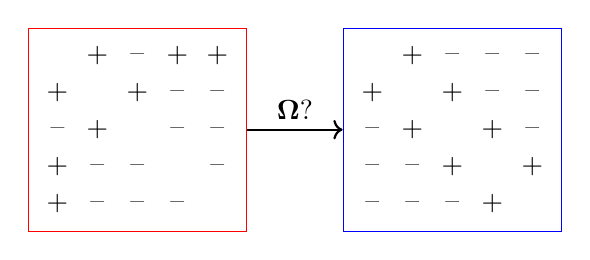
\begin{tikzpicture}
        \node[matrix,draw=red] (J0) at (-2,0)
        {
            & \node{+}; & \node{--}; & \node{+}; & \node{+}; \\
            \node{+}; &  & \node{+}; & \node{--}; & \node{--}; \\
            \node{--}; & \node{+}; &  & \node{--}; & \node{--}; \\
            \node{+}; & \node{--}; & \node{--}; &  & \node{--}; \\
            \node{+}; & \node{--}; & \node{--}; & \node{--}; &  \\
        };
        \node[matrix,draw=blue] (Jt) at (2,0)
        {
             & \node{+}; & \node{--}; & \node{--}; & \node{--}; \\
            \node{+}; &  & \node{+}; & \node{--}; & \node{--}; \\
            \node{--}; & \node{+}; &  & \node{+}; & \node{--}; \\
            \node{--}; & \node{--}; & \node{+}; &  & \node{+}; \\
            \node{--}; & \node{--}; & \node{--}; & \node{+}; & \\
        };
        \draw [->,black,thick] (J0.east) -- (Jt.west) node [above,midway] {$\mathbf{\Omega}$?};
    \end{tikzpicture}
    \caption{\label{fig:sign_structure} Determining the infeasibility of a target coupling graph}
\end{figure}




\appendix{\emph{Supplementary Information}}


\SetCoordinates[yAngle=90,xAngle=0]
\begin{figure}[h!]
    \begin{tikzpicture}
        \Vertices[NoLabel, size=.2, opacity=.9, style={shading=ball,blue}]{Data/spin_ladder_12_residual.csv}    
        \Edges[RGB]{Data/edges_spin_ladder_12_residual.csv}
    \end{tikzpicture}
    \caption{\label{fig:ladder}(a) Ladder with frustration. Top: near-neighbor couplings, bottom: residual couplings}
\end{figure}


\SetCoordinates[yAngle=90,xAngle=0]
\begin{figure}[h!]
    \begin{tikzpicture}
        \Vertices[NoLabel, size=.2, opacity=.9, style={shading=ball,blue}]{Data/AFM_triangularvertices_residual.csv}    
        \Edges[RGB]{Data/AFM_triangularedges_residual.csv}
    \end{tikzpicture}
    \caption{\label{fig:ladder}(a) Ladder with frustration. Top: near-neighbor couplings, bottom: residual couplings}
\end{figure}



\appendix{Experimental considerations}

\subsection{Experimentally Relevant parameters}

In order to significantly alter the phonon spectrum of a trapped ion crystal, the dipolar interaction due to the optical tweezers has to compete with the generally much stronger monopole interaction due the Paul trap. It is therefore beneficial to reduce the strength of the Paul trap as much as possible. However, in order for the spin-spin interactions to be properly mediated by the Raman laser, the ions have to be in the so-called Lamb-Dicke regime~\cite{James:1998} in which the ionic wavepacket is much smaller than the wavelength of the light, $\eta \sim k\sqrt{\hbar/(2m\omega_m)}\ll 1$, with $k$ the (effective) wavenumber of the laser inducing the spin-spin interactions. For Yb$^+$ excited near the D1 transition at 369~nm with a laser angle of 90~$^{\circ}$, we get a Lamb-Dicke parameter of $\eta \sim 0.2$ at $\omega_m = 2\pi$~400~kHz. Reducing the angle between the Raman beams further allows for reaching deeper in the Lamb-Dicke regime at even lower phonon frequencies at the expense of reducing the speed of the quantum simulator in order to reduce off-resonant coupling. We conclude that we require optical potentials with local trapfrequencies in the 100-400~kHz range to make meaningful changes to the phonon spectrum while maintaining the Lamb-Dicke regime.

To test the feasibility of changing the local trap frequency on this scale, we estimate the effect of a single tweezer. Taking Yb$^+$, and an experimentally feasible tweezer power of $P = 1$ W, a waist of $W_0 = 1 $ $\mu$m and wavelength $\lambda = 1060$~nm, we obtain local trapfrequencies due to the tweezers of $\sim 2\pi\cdot$~200~kHz. \rg{PLEASE SOMEBODY CHECK THESE NUMBERS}
\ASN{This can be a table...} \rg{Yes, perhaps}

Each optical tweezer will introduce a differential ac-Stark shift between the qubit states of the pinned ions and lead to off-resonant scattering. Both processes can lead to phase shifts \cite{Uys2010,Haeffner2003} on the state of the system which affect the performance of quantum operations \cite{Erhard2019} and can lead to decoherence. In the case of \(^{171}\text{Yb}^+\), we are concerned about both effects on the qubit states encoded on the hyperfine levels \(\ket{\text{F}=0,m_\text{F}=0}\equiv\ket{0}\) and \(\ket{\text{F}=1,m_\text{F}=0}\equiv\ket{1}\) of the \(^2\text{S}_{1/2}\) ground state. 

%For a strongly confining, red-detuned tweezer (\(\Omega_\text{p}=1.34\;\text{MHz},\; \lambda = 1024\) nm \rg{THere is no $2\pi$ in $\Omega_\text{p}$?)}, the scattering rate is \(\ll 1\) Hz (Fig. \ref{fig:scattering_rate}(a)) meaning that for quantum operations faster than 1~s the effect of off-resonant scattering is negligible.

The photon scattering rate in the center of the Gaussian tweezer beam with waist $W_0$ and peak intensity $I(0) = 2P/\pi W_0^2$ with total light power $P$ is approximately~\cite{Grimm:2000}
\begin{equation}
    \Gamma_{sc}(\omega) = \frac{3 c^2}{ \hbar\omega_0^3} \left(\frac{\omega}{\omega_0}\right)^3 \left(\frac{\Gamma}{\omega_0 - \omega} + \frac{\Gamma}{\omega_0 + \omega}\right)^2 \frac{P}{W_0^2}.
\end{equation} 

Only considering contributions from the D1 and D2 transitions in Yb$^+$, for $P = 1$ W, $W_0 = 1 $ $\mu$m and wavelength $\lambda = 1060$~nm, the photon scattering rate for the transitions of Yb$^{+}$ at $369$ nm ($\Gamma = 2\pi \cdot $19.65 MHz) and $329$ nm ($2 \pi \times  25.88$ MHz \cite{lifetimes}) is $2 \pi \cdot $2.5 Hz and $ 2 \pi \cdot 1.6$ Hz, respectively. We give an overview of the photon scattering rate in Fig.~\ref{fig:scattering_rate}(a). We conclude that it is possible to modify the phonon spectrum of trapped ions within the Lamb-Dicke regime and maintain negligible photon scattering on timescales of~$\sim$~100~ms. 

The main contribution to the differential Stark shift arises from off-resonant dipole couplings between the qubit states and hyperfine levels of the \(^2\text{P}_{1/2}\) and \(^2\text{P}_{3/2}\) states. Since we consider the ground clock states of $^{171}$Yb$^+$ as qubits the differential Stark shift is highly suppressed as compared to the common Stark shift~\cite{Lee:2005}. It is dominated by the 12.6~GHz Hyperfine splitting that causes a difference in detuning between the two states~\cite{Hirzler:2020,Teoh2021}. For $P = 1$ W, $W_0 = 1 $ $\mu$m and wavelength $\lambda = 1060$~nm, we obtain a differential Stark shift of XXXX~Hz (Fig.~\ref{fig:scattering_rate}(b)). 

Since the tweezer pattern is in general not homogeneous, they will cause local variations in AC Stark shifts that will appear as an inhomogeneous additional field in the quantum simulator. For certain ion species and qubit states, such in as Ca$^+$, the differential Stark shift can be eliminated by using tweezers operating at a magic wavelength or polarizability, however for the ground state qubit of $^{171}\text{Yb}^{+1}$ these are not available. An alternative is to use pairs of blue and red detuned tweezers such that the combined differential Stark shift becomes zero. In Fig.~\ref{fig:stark_compensation} we show an example using tweezers operating at 532 and 224 nm.

As a more elegant solution to eliminate differential Stark shifts, we propose the following. The trapfrequency due to a tweezer intensity pattern around ion $i$, $I_i=I(\vec{r}_i)$ scales as $\Omega^2_i\propto P_i/w_0^4$ with $P_i$ the local power in the tweezer. In contrast, the differential Stark shift scales as $\Delta_\text{AC}\propto P_i/w_0^2$. Therefore, we can make the differential Stark shift between the qubit states homogeneous throughout the ion crystal by controlling not only the power $P_i$ of each tweezer but also each waist $w_i$ and assuring that $P_i/w_i^2$ is constant around each ion. This solution still gives us complete freedom to engineer each local tweezer trap frequency, but comes at the expense of having in general stronger laser power requirements.




\rg{PLEASE SOMEBODY CHECK THESE NUMBERS}








\begin{figure}[h!]
    \begin{tikzpicture}
        \begin{groupplot}[group style={group size=2 by 1, horizontal sep=0.1\textwidth}]
            \nextgroupplot[
                ymode=log,
                height=0.245\textwidth,
                width=0.245\textwidth,
                xtick = {250,500,750,1000},
                xlabel={$\lambda\; (\text{nm})$},
                ylabel={$\Gamma\; (\text{Hz})$}
                ] 
                \addplot [mark=none, very thick] table[x index=0, y index=1]{Data/scattering_rate.txt};
                \node [anchor=north west] at (rel axis cs:0,1) {(a)};
            \nextgroupplot[
                    height=0.245\textwidth,
                    width=0.245\textwidth,
                    xlabel = $\Delta_{\text{AC}}\;(\text{Hz})$,
                    ylabel = $\Omega_p\; (\text{kHz})$,
                    xtick = {0,1000,2000}
                ]
                \addplot+[mark=none, very thick] table[x index=0, y index=1]{Data/stark_shift_vs_pin_freq.txt};
                %\addplot+[mark=none, very thick] file[x index=0, y index=1]{Data/stark_shift_vs_pin_freq_224.txt};
                \node [anchor=north west] at (rel axis cs:0,1) {(b)};
        \end{groupplot}
    \end{tikzpicture}
    \caption{\label{fig:scattering_rate}(a) Scattering rate of Yb$^{+1}$, (b) Stark shifts and pinning frequencies from a tightly focused tweezer (\(w_0=2\; \upmu\)m) at 1070 nm for a laser power of (a) 1 W and (b) 10 to 1000 mW and linear polarization}
\end{figure}




\begin{figure}[h!]
    \begin{tikzpicture}
        \begin{groupplot}[group style={group size=2 by 1, horizontal sep=0.1\textwidth}]
            \nextgroupplot[
                legend style={
                at={(1,0.6)},
                anchor=east},
                xmax = 400,
                height=0.245\textwidth,
                width=0.245\textwidth,
                xlabel = $\Delta_{\text{AC}}\;(\text{Hz})$,
                ylabel = $\Omega_p\; (\text{kHz})$,
                xtick = {0,200,400}
            ]
            \addplot+[mark=none, very thick] table[x index=0, y index=1]{Data/stark_shift_vs_pin_freq_532.txt};
            \addplot+[mark=none, very thick] table[x index=0, y index=1]{Data/stark_shift_vs_pin_freq_224.txt};
            \node [anchor=north west] at (rel axis cs:0,1) {(a)};
            \legend{532 nm,224 nm}
            \nextgroupplot[
                title={$P_\text{532}\;(\text{W})$},
                height=0.245\textwidth,
                width=0.245\textwidth,
                xlabel = $P_\text{224}\;(\text{W})$,
                ylabel = $\Omega_p\; (\text{kHz})$,
                extra x ticks={0,0.5,1},
                extra x tick style={%
                    ,grid=major
                    ,ticklabel pos=top
                    },
                extra x tick labels={0,0.06,0.12}
                ]
            ]
            \addplot+[mark=none, very thick] table[x index=0, y index=1, col sep=tab]{Data/stark_shift_compensation.txt};
            \node [anchor=north west] at (rel axis cs:0,1) {(b)};
        \end{groupplot}
    \end{tikzpicture}
    \caption{\label{fig:stark_compensation}(a) Stark shifts and pinning frequencies from a tightly focused tweezer (\(w_0=2\; \upmu\)m) at 224 and 532 nm for a laser power of 1 W and (b) combined pinning frequency for tweezer pair with zero ac-Stark shift.}
\end{figure}



\rg{It would be nice to have a small section on missalligning the tweezers (basically Lisa's project but perhaps we can run a quick sim?)}

\section{Physical picture}

Effect of a single potential

\begin{figure}[h!]
    \begin{subfigure}{0.5\textwidth}
        \subcaptionbox{\label{label1}}
        {\begin{tikzpicture}[baseline]
            \Vertices[size=.2, opacity=.9, style={shading=ball,blue}]{Data/Ladder_sensitivityvertices.csv}    
            \Edges[NoLabel,RGB]{Data/Ladder_sensitivityedges.csv}
            \node [circle, anchor=north west, draw=red, very thick, dotted] at (-0.31,-0.29) {};
        \end{tikzpicture}}
    \end{subfigure}
    \begin{subfigure}{0.5\textwidth}
        \subcaptionbox{\label{label2}}
        {\begin{tikzpicture}[baseline]
            \Vertices[size=.2, opacity=.9, style={shading=ball,blue}]{Data/Ladder_sensitivityvertices_residual.csv}    
            \Edges[NoLabel, RGB]{Data/Ladder_sensitivityedges_residual.csv}
        \end{tikzpicture}}
    \end{subfigure}
    \pgfplotscolorbardrawstandalone[colormap={}{of colormap={PRGn,},},
        point meta min=-1,
        point meta max=1,
        colorbar horizontal,
        colormap access=map,
        colorbar style={
        width=2cm, height=0.2cm, font=\tiny},
        ]
        \caption{\label{fig:pin_gradient} Gradient of coupling}
\end{figure}


%\bibliographystyle{apa}
\bibliography{TweezerIon}



\end{document}
